\chapter{Wprowadzenie teoretyczne}

\section{Roboty mobilne}

Robot mobilny to autonomiczny pojazd zdolny do poruszania się po swoim środowisku, bez fizycznego przywiązania do jednej lokalizacji \cite{mobile_robot}. Oznacza to, że ich przestrzeń robocza jest konstrukcyjnie nieograniczona, nie posiada ograniczeń takich jak np. przewodowy sterujące podłączone stacjonarnie do jednego miejsca. Dodatkowo nie wymagają one bezpośredniej ingerencji człowieka. Sprawia to, że ich konstrukcja mechaniczna może przyjmować dowolne rozmiary potrzebne do wykonywanych zadań, bez ograniczeń związanych z czynnikiem ludzkim. 

Środowiskiem robota mobilnego może być ląd, woda lub powietrze. W oparciu o środowisko poruszania się, roboty mobilne można podzielić na:

\begin{itemize}
\item
 \textit{Jeżdżące}
 \item
 \textit{Kroczące}
 \item 
 \textit{Pływające}
 \item 
 \textit{Latające} 
 \item 
 \textit{Inne}
\end{itemize}

 Najbardziej popularną grupą są roboty jeżdżące. Grupa ta rozwija się w szybkim tempie, jest to spowodowane między innymi inwestycjami globalnych koncernów motoryzacyjnych. Skupiają się one na rozwoju technologicznym i dążą do coraz większej autonomiczności swoich pojazdów. Prekursorem w tej dziedzinie jest firma Tesla, która zapowiedziała, że  w połowie 2020 roku, w ich pojazdach zostanie wprowadzony tryb pełnej autonomicznej jazdy. 
 
 Ze względu na dynamiczny rozwój tej grupy robotów mobilnych, są one też popularne pośród konstruktorów-amatorów, którzy zajmują się budową robotów w celach dydaktycznych, badawczych lub hobbistycznych.  
\section{Napęd różnicowy}

 Napęd różnicowy umożliwia kołom na jednej osi uzyskanie różnych prędkości obrotowych, jest to niezbędne w przypadku robotów o napędzie kołowym bez skrętnej osi. Podczas ruchu po łuku, koła pojazdu pokonują inną drogę. Zastosowanie napędu różnicowego pozwala, aby toczyły się one po swoich torach ruchu bez poślizgu, osiągając różne prędkości obrotowe.
\section{Robot Operating System}

ROS(Robot Operating System) jest to meta-operacyjny systemem dla robotów, który posiada otwarty dostęp do kodu źródłowego. Podobnie jak zwyczajny system operacyjny zapewnia warstwę abstrakcji sprzętowej, kontrolę urządzeń niskopoziomowych, implementacje powszechnie używanych funkcjonalności \cite{ROS}. ROS różni się jednak od powszechnego systemu, możliwością komunikacji między wątkowej. Procesy mogą komunikować się ze sobą w czasie swojego wykonywania. Sprawia to, że ROS jest dobrym systemem do wsparcia sterowania robotem oraz czujnikami(Rys.\ref{fig:ROS_meta_system}). Kolejną zaletą systemu ROS jest możliwość współpracy z większością popularnych systemów operacyjnych takich jak Windows, Linux, Mac, Android lub iOS. 

\begin{figure}[ht]
	\centering
	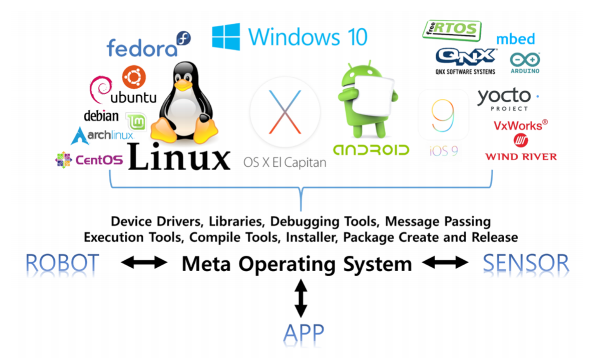
\includegraphics[scale=1]{ROS_meta_system.png}
	\caption{ROS jako meta-operacyjny system \cite{ROS}.}
	\label{fig:ROS_meta_system}
\end{figure}

Główne założenia sytemu ROS można przedstawić jako \cite{ROS_goals}:

\begin{itemize}
	\item 
	\textit{Komunikacja P2P(peer to peer)} - model komunikacji w sieci komputerowej zapewniający wszystkim hostom te same uprawnienia \cite{P2P}.
	\item
	\textit{Oparty na narzędziach} - duża liczba małych narzędzi jest używana do budowania i uruchamiania różnych komponentów systemu.
	\item 
	\textit{Wielojęzykowy} - wspiera wiele języków programowania.
	\item 
	\textit{Niezagnieżdżony} - tworzenie tylko małych plików wykonywalnych, które ujawniają bibliotekę funkcjonalności do systemu ROS. Pozwala to na łatwiejszą ekstrakcję kodu i użycie go ponownie poza pierwotnym przeznaczeniem.  
	\item 
	\textit{Darmowy i posiadający otwarty dostęp do kodu źródłowego.}
\end{itemize}

\begin{figure}[ht]
	\centering
	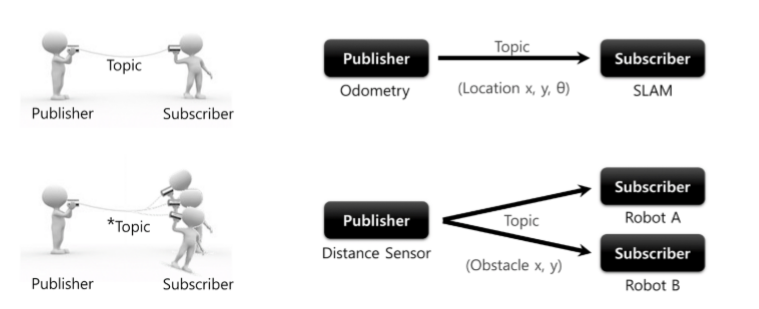
\includegraphics[scale=0.8]{topic.png}
	\caption{Komunikacja z wykorzystaniem tematów. \cite{ROS}.}
	\label{fig:topic}
\end{figure}

Komunikacja odbywa się między \textit{węzłami(ang. nodes)}, czyli pojedynczymi procesami działającymi w ramach systemu ROS. Kanał komunikacyjny między węzłami to \textit{temat(ang. topic)}. \textit{Wiadomość(ang message)} to dane wysyłane między węzłami za pomocą tematu. Węzeł publikuje lub subskrybuje temat, czyli wysyła lub pobiera z niego wiadomość. Schemat komunikacji przy pomocy tematów został przedstawiony na Rys.\ref{fig:topic}.




\section{TurtleBot}

Turtlebot jest standardowym robotem platformowym wykorzystującym komunikację między wątkową ROS. Platforma ta jest bardzo popularna wśród deweloperów, a także studentów, ponieważ doskonale nadaje się do celów dydaktycznych. Oprogramowanie posiada otwarty dostęp do kodu źródłowego \cite{turtlebot3}. Upraszcza to zrozumienie zasady działania platformy, ponieważ umożliwia łatwy dostęp do dokumentacji, w której znajduje się opis działania poszczególnych modułów. 

\begin{figure}[ht]
	\centering
	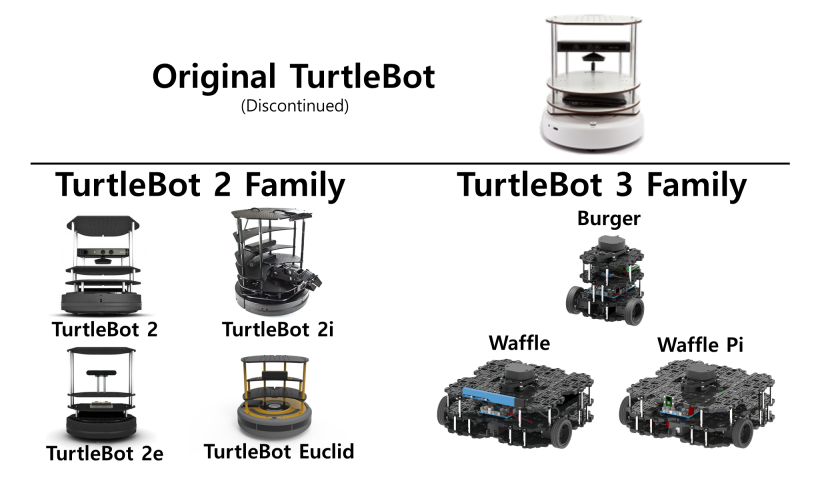
\includegraphics[scale=0.7]{turtlebot.png}
	\caption{Rodzina robotów TurtleBot. \cite{turtlebot}.}
	\label{fig:turtlebot}
\end{figure}  

Istnieją trzy wersje robotów serii TurtleBot(Rys.\ref{fig:turtlebot}). Najnowsza z nich została zaprezentowana w maju 2017 roku. TurtleBot3 jest małym, niskobudżetowym, programowalnym, opartym na komunikacji między wątkowej ROS robotem mobilnym, który służy do celów edukacyjnych, badawczych lub hobbistycznych.  Składa się on z wewnętrznego komputera, mikro kontrolera, systemu wizyjnego i czujników.  Wewnętrzny komputer komunikuje się przy pomocy komunikacji ROS przez WiFi ze zdalnym komputerem. Udostępnia on dane z czujników i otrzymuje sterowanie, czyli prędkość liniową i kątową, która jest następnie przeliczana na wartość prędkości obrotowej każdego z kół. Mikro kontroler komunikuje się z komputerem wewnętrznym przy pomocy szeregowej komunikacji między wątkowej. 


